\documentclass[11pt]{article}

\usepackage[margin=1in]{geometry}
\usepackage{amsmath,amssymb,amsthm,mathrsfs}
\usepackage{graphicx}
\usepackage[hidelinks]{hyperref}

\newtheorem{theorem}{Theorem}

\newcommand{\B}{\mathscr{B}}
\newcommand{\G}{\mathscr{G}}
\newcommand{\K}{\mathscr{K}}
\newcommand{\N}{\mathbb{N}}
\newcommand{\Sch}{\mathcal{S}}
\newcommand{\Sing}{\mathscr{S}}
\newcommand{\cnull}{c_0}

\begin{document}

\begin{center}
{\Large Literature status: strictly singular operators and \(c_0\)-factorization on Schreier spaces}

\medskip
{\small Run \texttt{fa\_banach\_001}; source arXiv:1907.10645}
\end{center}

\section*{Source question}

Beanland, Kania, and Laustsen study the closed ideal lattice of
\(\B(X)\) when \(X\) is Tsirelson's space or a finite-order Schreier space.
In Section 5 of \cite{BKL}, for \(X=X[\Sch_n]\), \(n\geq 1\), they write
\(\overline{\G}_{c_0}(X)\) for the norm closure of the ideal of operators on
\(X\) that factor through \(c_0\).  They observe that
\[
  \overline{\G}_{c_0}(X)
  \subseteq
  \bigcap\{ \mathscr{I} : \mathscr{I}\text{ is a non-trivial spatial ideal of }\B(X)\},
\]
and then ask, among other things, whether
\[
  \Sing(X)\subseteq \overline{\G}_{c_0}(X).
\]

\begin{figure}[h]
\centering

\includegraphics[width=\textwidth]{figures/open_problem_crop.png}
\caption{arXiv:1907.10645, page 22: the source question about
\(\Sing(X)\subseteq \overline{\G}_{c_0}(X)\) for \(X=X[\Sch_n]\).}
\end{figure}

\section*{Supporting literature status}

Manoussakis and Pelczar-Barwacz later studied small closed ideals on the
Schlumprecht and Schreier spaces.  In Section 4.2 of \cite{MPB}, they
explicitly say that for finite-order Schreier spaces \(X[\Sch_N]\), the
reverse inclusion fails when \(N\geq 2\), answering one of the questions of
\cite{BKL}; they also state that the case \(N=1\) remains open.

\begin{figure}[h]
\centering
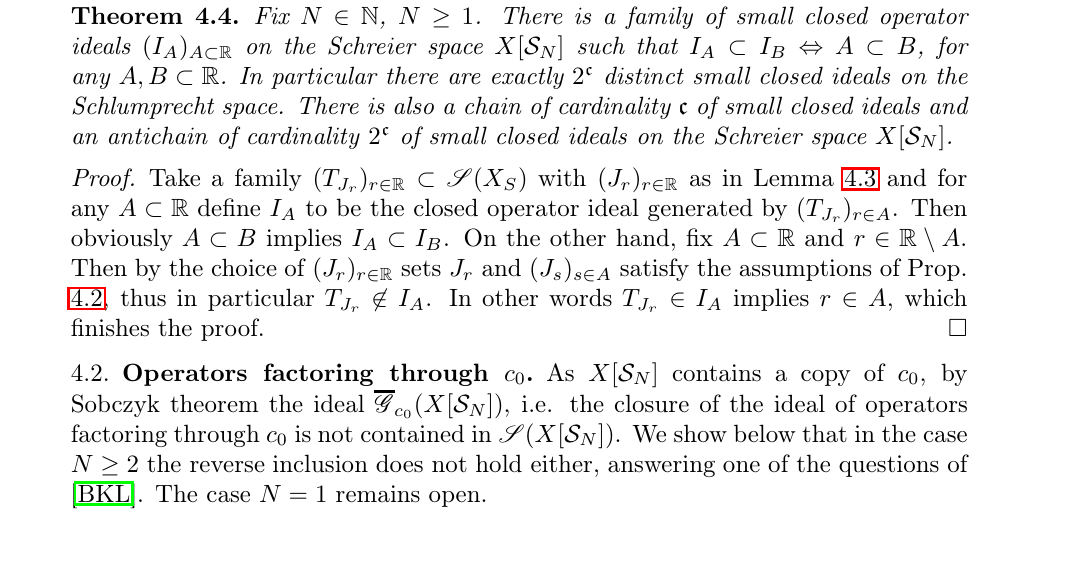
\includegraphics[width=\textwidth]{figures/supporting_answer_setup_crop.png}
\caption{arXiv:2008.12362, page 14: the later paper states that the reverse
inclusion fails for \(N\geq 2\), answering one of the questions of
\cite{BKL}, while \(N=1\) remains open.}
\end{figure}

\begin{figure}[h]
\centering

\includegraphics[width=\textwidth]{figures/supporting_answer_crop.png}
\caption{arXiv:2008.12362, page 16: Corollary 4.7 gives
\(\Sing(X[\Sch_N])\not\subset \overline{\G}_{c_0}(X[\Sch_N])\) for \(N\geq 2\).}
\end{figure}

\section*{Proof intuition}

The source question asks whether every strictly singular operator on a
finite-order Schreier space lies in the closed ideal generated by operators
factoring through \(c_0\).  The later paper finds a canonical obstruction:
the formal identity \(R_N:X[\Sch_N]\to X[\Sch_{N-1}]\).  It is strictly
singular, but for \(N\geq 2\) it cannot be approximated within distance one
by any composition through \(c_0\).  Thus \(R_N\) is a strictly singular
operator that remains outside \(\overline{\G}_{c_0}(X[\Sch_N])\).

\section*{The literature answer}

\begin{theorem}
For every \(N\in\N\) with \(N\geq 2\),
\[
  \Sing\bigl(X[\Sch_N]\bigr)
  \not\subset
  \overline{\G}_{c_0}\bigl(X[\Sch_N]\bigr).
\]
Consequently, the inclusion question from \cite{BKL} has a negative answer
for finite-order Schreier spaces of order at least two.
\end{theorem}

\begin{proof}
Manoussakis and Pelczar-Barwacz prove in Proposition 4.6 of \cite{MPB} that
the formal identity
\[
  R_N:X[\Sch_N]\longrightarrow X[\Sch_{N-1}]
\]
is strictly singular for every \(N\geq 1\).  They further prove that, if
\(N\geq 2\), then for every pair of bounded operators
\[
  T:X[\Sch_N]\to c_0,
  \qquad
  S:c_0\to X[\Sch_{N-1}],
\]
one has
\[
  \|R_N-S\circ T\|\geq 1.
\]

This says precisely that \(R_N\) cannot be approximated by operators that
factor through \(c_0\).  Since \(R_N\) is strictly singular, \(R_N\) gives an
element of \(\Sing(X[\Sch_N])\) that does not belong to
\(\overline{\G}_{c_0}(X[\Sch_N])\).  Corollary 4.7 of \cite{MPB} records the
result explicitly:
\[
  \Sing(X[\Sch_N])\not\subset \overline{\G}_{c_0}(X[\Sch_N])
  \qquad (N\geq 2).
\]
\end{proof}

\section*{Verification notes and limitations}

This packet is a literature-status identification, not a new proof from the
run.  The supporting paper explicitly identifies the result as answering one
of the questions of \cite{BKL}.  The evidence crops above show both the source
question and the later answer/corollary.

The result is a partial subcase of the Section 5 questions in \cite{BKL}.  It
does not settle \(N=1\); \cite{MPB} explicitly leaves that case open.  It also
does not decide whether
\(\overline{\G}_{c_0}(X)\) is properly contained in the intersection of all
non-trivial spatial ideals, nor does it describe explicit maximal ideals in
\(\B(T)\) or \(\B(X[\Sch_n])\).

Before promotion, the run lightweight indexes were searched for arXiv:1907.10645,
the title phrase, ``closed ideals of operators'', ``Tsirelson'', ``Schreier'',
``operator ideals'', and nearby core terms.  No existing exact packet or
attempt was found.  Local source search and web search then identified
arXiv:2008.12362 as the relevant later paper.

\section*{Human review recommendation}

Treat the source question \(\Sing(X)\subseteq\overline{\G}_{c_0}(X)\) as
already answered negatively for \(X=X[\Sch_N]\), \(N\geq 2\), by
\cite{MPB}.  Keep the \(N=1\) case and the other open questions from the
source Section 5 separate.

\begin{thebibliography}{9}

\bibitem{BKL}
K. Beanland, T. Kania, and N. J. Laustsen,
\emph{Closed ideals of operators on the Tsirelson and Schreier spaces},
J. Funct. Anal. 279 (2020), 108668; arXiv:1907.10645.

\bibitem{MPB}
A. Manoussakis and A. Pelczar-Barwacz,
\emph{Small operator ideals on the Schlumprecht and Schreier spaces},
arXiv:2008.12362.

\end{thebibliography}

\end{document}
